\documentclass[a4paper,10pt]{article}
\usepackage[utf8x]{inputenc}
%\usepackage[utf8]{inputenc}
\usepackage{graphicx}
\usepackage{color}
\usepackage[table]{xcolor}
\usepackage{url}
\usepackage{enumitem}% http://ctan.org/pkg/enumitem
%\usepackage{algorithm, algorithmicx}
\usepackage[noend]{algpseudocode}
\usepackage{comment}
\usepackage[standard]{ntheorem}
\usepackage{multirow}
\usepackage{subcaption}
\usepackage{caption}
\usepackage[noadjust]{cite}
\usepackage{pdflscape}
\usepackage{lipsum}
\usepackage{capt-of}
\usepackage[linesnumbered,ruled,vlined]{algorithm2e}
\usepackage{amsmath,amssymb,amsfonts}
\usepackage{threeparttable}
\usepackage{booktabs}
\newtheorem{notation}{Notation}


\setlength{\textheight}{9.2in}
\setlength{\textwidth}{6.4in}

\setlength{\oddsidemargin}{0mm}
\setlength{\evensidemargin}{0mm}
\setlength{\topmargin}{-0.3in}

\newcommand{\sat}{$\;\triangleleft\;$}
\newcommand{\nsat}{$\;\ntriangleleft\;$}

\newcommand{\subgraphname}{part}
\newcommand{\subgraphnamespace}{part }
\newcommand{\subgraphnameCaps}{Part}

\usepackage[bookmarks=false]{hyperref}
\hypersetup{
	colorlinks,
	citecolor=black,
	filecolor=black,
	linkcolor=black,
	urlcolor=black
}
\graphicspath{{./images/}{./lstmResults/}{./cnnResults/}{./somResults}}
\usepackage{mathtools}
\DeclarePairedDelimiter{\ceil}{\lceil}{\rceil}
\DeclarePairedDelimiter\floor{\lfloor}{\rfloor}
\newcommand{\numBytesOffChip}{\mathbb{B}}
\newcommand{\numOverlap}{\delta}
\newcommand{\busWidth}{BW}
\newcommand{\dataWidth}{DW}
\newcommand{\dataLength}{l}
\newcommand{\addressSym}{Addr}
\newcommand{\BuffSize}{buffSize}
%\newcommand{\EXPANDER}{{\scriptsize  {EXPANDER}}\xspace}

\begin{document}
	
\begin{titlepage}
	
	\begin{center}
		
		\vspace{4cm}
%		\LARGE \textbf{A FRAMEWORK FOR MAPPING NEURAL NETWORKS ON PARALLEL ARCHITECTURES}\\
	\LARGE \textbf{OPTIMIZING NEURAL NETWORKS PERFORMANCE  ON PARALLEL ARCHITECTURES}\\		
		\vspace{2cm}
		
		\large {A synopsis submitted in partial fulfillment of the requirements for the degree\ \\}
		\vspace{0.5cm}
		\large {of\ \\}
		\vspace{0.5cm}
		\Large \textbf{Doctor of Philosophy \ \\}
		\vspace{0.5cm}
		
		\large \ \\ \ \\ Submitted by: \ \\
		\Large \textbf{SAURABH TEWARI \ \\ (2015CSZ8046)} 
		
		\large {\ \\ under the guidance of \ \\}
		% \vspace{0.2cm}
		\large \textbf{ Prof. Anshul Kumar\\ }
		\large \textbf{ Prof. Kolin Paul\\ }
		% \large {Department of Computer Science and Engineering \ \\}
		\vspace{2.0cm}
		\hspace{0cm}
		\includegraphics[scale=1.0]{images/logo.pdf} \\
		\vspace{2.0cm} 
		\Large {DEPARTMENT OF COMPUTER SCIENCE \& ENGINEERING}\\
		\Large {INDIAN INSTITUTE OF TECHNOLOGY DELHI \\ NEW DELHI}\\
		% \vspace{2cm}
	\end{center}
	
\end{titlepage}
\pagenumbering{roman}
\section*{List of Included Papers}
This thesis is based on the following publications:

\textbf{Published:}

\newcounter{saveenum}

\begin{enumerate}
\item \textbf{S. Tewari}, A. Kumar and K. Paul, ``\textit{SACC: Split and Combine Approach to Reduce the Off-chip Memory Accesses of LSTM Accelerators}'', in DATE 2021.

\item \textbf{S. Tewari}, A. Kumar and K. Paul, ``\textit{Minimizing Off-Chip Memory Access for CNN Accelerators}'', in IEEE Consumer Electronics Magazine 2021.

\item \textbf{S. Tewari}, A. Kumar and K. Paul, ``\textit{Bus Width Aware Off-Chip Memory Access Minimization for CNN Accelerators}", in ISVLSI 2020.

\item D. Stathis, Y. Yang, \textbf{S. Tewari}, A. Hemani, K. Paul, M. Grabherr and R. Ahmad, ``\textit{Approximate Computing Applied to Bacterial Genome Identification using Self-Organizing Maps}'', in ISVLSI 2019.

\setcounter{saveenum}{\value{enumi}}
\end{enumerate}



%\textbf{In-review/Under preparation:}
%\begin{enumerate}
%  \setcounter{enumi}{\value{saveenum}}
%
%\item \textbf{Rajesh Kedia}, Shikha Goel, M. Balakrishnan, Kolin Paul, and Rijurekha Sen. ``\textit{Design space exploration of FPGA based system with heterogeneous DNN accelerators}''. Submitted to IEEE Embedded Systems Letters.
%
%\item \textbf{Rajesh Kedia}, M. Balakrishnan, and Kolin Paul. ``\textit{An integrated flow for designing Context-aware Adaptive Embedded Systems}'' -- under preparation.
%
%\item Shikha Goel, \textbf{Rajesh Kedia}, M. Balakrishnan, and Rijurekha Sen. ``\textit{INFER: INterFerence-aware Estimation of Runtime for concurrent DNN execution on DPUs}'' -- under preparation.
%
%\end{enumerate}




\newpage
\setcounter{tocdepth}{2}
\tableofcontents
\newpage

\pagenumbering{arabic}
\begin{comment}
	1. Introduction - 2 pages
	2. Related work - 0.5 pages
	3. Overall flow - 0.75 pages
	4. Graphical representation - 2 pages
	5. DSE flow - 2 pages
	6. Runtime controller generation - 1.5 page
	7. Case studies - 3.5 pages
	a. RBD - (0.5 page)
	b. MAVI - (2 pages)
	c. DPU - (1 page)
	8. Conclusion - 0.5 page
	9. References - 2 pages
\end{comment}
\section{Introduction}
The past few years have seen a rapid growth in Neural Network (NN) based applications. These are widely used in healthcare, agriculture, road safety, surveillance, defense, and others. Modern computing systems capable of storing and processing large volumes of data, and the availability of big data sets, have enabled NNs to achieve human-like performance, which was not possible a few decades ago.

Neural Networks are machine learning algorithms inspired by processing mechanisms in the human brain. These consist of several neurons connected and organized as layers. \figurename{~\ref{fig:simpleNN}} shows a simple NN example. Each layer has weights and biases, learned using the training process. Once trained, these weights and biases are used in the applications for inferencing. There are several classes of NNs that differ from each other in the number of neurons, connections between them, and method of training. 
\begin{figure}[!htb]
	\centering
    \captionsetup{font=sf}
	\subfloat[]
	{\includegraphics[width=0.2\textwidth]{simpleFFNN}
		\label{fig:simpleNN}}
	\hfil
	\subfloat[]
	{\includegraphics[width=0.4\textwidth]{nnClassification}
		\label{fig:nnClassification}}
	\hfil
	\caption{(a) Example of simple Neural Network. (b) Broad categories of NNs.}
	\label{fig:intro}
\end{figure}

\figurename{~\ref{fig:nnClassification}} shows two broad classes of NNs, feedforward neural networks (FFNNs) and recurrent neural networks (RNNs). In FFNNs, the data flows from the input layer to the output layer via intermediate layers, and there are no loops. These can be represented as directed acyclic graphs. FFNNs do not have any internal state, and output depends on the current input and the parameters. Based on the number of layers, FFNNs can be further classified as single-layer and multi-layer FFNNs. Single-layer Feedforward NNs consist of just two layers - an input and an output layer. Only the output layer performs computation. Self-Organizing Maps (SOMs) are examples of single-layer NNs and are used in dimensionality reduction and clustering applications. 

Multilayer FFNNs represent the most important class of machine learning algorithms. They consist of one or more intermediate layers (hidden layers) between the input and output layers. Depending on whether the neurons in the layer are connected to all or a few of the neurons in the previous layers, these can be further classified as fully connected FFNNs (\figurename{~\ref{fig:fullyConnected}}) or sparsely connected FFNNs (\figurename{~\ref{fig:sparselyConnected}}), respectively. One of the most popular class of FFNNs used for image classification and recognition from images is Convolutional Neural Networks (CNNs).

Another popular class of NNs is recurrent neural networks (RNNs), which have layers with loops (\figurename{~\ref{fig:recurrentLayer}}). These networks extract information from the inputs and store it in an internal state. In this class of NNs, the output depends not only on the current input but also on the internal state. These networks are widely used in speech recognition, natural language processing (NLP), and other sequential data processing applications. Long short-term memory networks (LSTMs) are among the popular variants of RNNs.

\begin{figure}[!htb]
	\centering
    \captionsetup{font=sf}
	\subfloat[]
	{\includegraphics[width=0.15\textwidth]{fullyConnected}
		\label{fig:fullyConnected}}
	\hfil
	\subfloat[]
	{\includegraphics[width=0.15\linewidth]{sparselyConnected}
		\label{fig:sparselyConnected}}
	\hfil
	\subfloat[]
	{\includegraphics[width=0.15\linewidth]{recurrentLayer}
	\label{fig:recurrentLayer}}
	\caption{Types of NN layers (a) Fully Connected FF. (b) Sparsely Connected FF. (c) Recurrent. }
	\label{fig:nnLayers}
\end{figure}

Multilayer NNs with more than three layers are referred to as deep neural networks (DNNs), capable of learning complex functions. Recently, DNN models with several hundreds of layers have been reported~\cite{he2016deep}. These DNNs have millions of parameters (weights and biases) and perform compute-intensive and memory-intensive operations. For learning, these DNNs require large training data sets, and need to go through multiple iterations to achieve the desired accuracy, requiring significant computational resources and time. Training of these large models is mainly performed on high-end servers and consume high energy. Once these models are trained, they are deployed in applications for inferencing, where the deployment platforms may range from cloud to embedded devices.

Manufacturers are shifting the processing of NNs from cloud to edge devices like smartphones and tablets to improve the user experience, eliminate network bandwidth issues, and improve privacy and security. These battery-operated edge devices have limited resources and a tight energy, budget which poses significant challenges. Efficient processing of DNNs inferencing on edge devices is critical for their widespread usage. In this work, we focused on the efficient processing of NNs inference on edge devices. 

Energy efficiency and throughput are the two most important metrics for edge devices. While energy efficiency is of paramount importance for longer battery time, high throughput is desired for better user-response time. Edge devices mostly use customized accelerators to meet energy and throughput demands. Several FPGA~\cite{zhang2015optimizing,wei2019overcoming,gokhale2014240,8742284,gupta2015deep,alwani2016fused}, GPU~\cite{chetlur2014cudnn} and ASIC~\cite{Chen2016EyerissAS,chen2014diannao,chen2014dadiannao,du2015shidiannao} accelerators have been proposed to meet the performance and energy targets. 
\begin{figure}[!htb]
	\centering
    \captionsetup{font=sf}
	\subfloat[]
	{\includegraphics[width=0.4\textwidth]{typicalDNNAccelerator}
		\label{fig:typicalDNNAccelerator}}
	\hfil
	\subfloat[]
	{\includegraphics[width=0.35\linewidth]{roofline}
		\label{fig:roofline}}
	\caption{(a) Typical DNN accelerator architecture. (b) Roofline model}
	\label{fig:acceleratorAndRoofline}
\end{figure}

\figurename{~\ref{fig:typicalDNNAccelerator}} shows a typical DNN accelerator architecture, which consists of an off-chip memory and an accelerator chip. An accelerator chip mainly consists of an on-chip memory of a few hundred KBs and an array of Processing Elements (PEs). The accelerator system has multiple memory levels: off-chip memory, on-chip memory, and the registers inside the PEs. Each memory level has different access latency and energy costs. The memory access energy from off-chip memory is up to two orders of magnitude higher than a PE computation operation~\cite{Chen2016EyerissAS}. It has been observed that more than 80\% of the overall energy consumption of these accelerators is due to off-chip memory accesses~\cite{chen2014diannao}. 

The PE-array (\figurename{~\ref{fig:typicalDNNAccelerator}}) has a large number of processing elements, capable of performing several operations per cycle. However, throughput is often limited by off-chip memory bandwidth~\cite{williams2009roofline}. Fig.~\ref{fig:roofline} shows attainable throughput in such a scenario as a function of the operational intensity of an application. The figure shows two application kernels (A and B) with different operational intensities (FLOPS/byte), with performance limited by the memory bandwidth in both cases, which is typically the case for most DNN accelerators. Kernel B, however, has better operational intensity than kernel A and achieves better throughput. Effective data-reuse techniques are required to improve the performance of bandwidth-limited parallel architectures. Therefore, reducing the off-chip memory is the key to improving the throughput and energy efficiency of DNN accelerators. Much recent research has focused on reducing off-chip memory accesses.
\begin{figure}[!htb]
	\centering
    \captionsetup{font=sf}
	\includegraphics[width=0.5\textwidth]{previousWorkClassification}
	\caption{Broad Classification of previous works for improving the performance of DNN accelerators.}
	\label{fig:previousWorkClassification}
\end{figure}

Recent works that aim to reduce the off-chip memory accesses of NN accelerators can be classified into two broad categories, as shown in Figure~\ref{fig:previousWorkClassification}. One category of work exploits error-tolerance and redundancy in NNs using quantization, compression, and pruning techniques to reduce the precision, the number of operations and models' size~\cite{ferreira2016fpga,wang2018c,chang2015recurrent,han2017ese,lee2016fpga}. With reduced precision, the storage requirement and memory accesses reduce proportionally and improve energy efficiency~\cite{sze2017efficient}. In shallow NNs, the number of parameters is smaller compared to DNNs. Quantization and pruning techniques result in reduced NN model sizes. The reduced model for shallow NNs may fit into the on-chip memory and thus eliminate the off-chip memory bandwidth bottleneck. However, quantization and pruning approaches impact the accuracy of the networks and may not be suitable where accuracy can not be compromised. Also, the number of parameters in modern DNNs is significantly large. For these DNNs, besides quantization and pruning, additional techniques are required to further reduce the off-chip memory accesses.

The other approach, which does not affect the accuracy of the network, is to reduce repeated off-chip accesses to the same NN coefficients when the entire set of NN coefficients does not fit in the on-chip memory. This is quite effective for many modern DNNs (e.g., CNNs, RNNs) with a significantly large number of parameters~\cite{zhang2015optimizing,Li2018SmartShuttleOO,que2019efficient,park2020time}. The weights are repeatedly used for all the inputs during the inference phase. Inputs can be grouped as a batch and processed to reuse the weights. This technique is referred to as batch processing. Increasing the batch size increases the weights reuse but also increases the latency. Another prominent data reuse technique is data partitioning and scheduling. In this technique, the data is partitioned into tiles, and operations on tiles are scheduled in such a way that data can be accessed from the on-chip memory, as far as possible. For a given DNN, there are numerous ways of doing data partitioning and scheduling, offering different extents of data reuse. Choosing an optimal way here is non-trivial.

The data-reuse approaches are orthogonal to the quantization techniques and can be combined to reduce the off-chip memory accesses further. In this work, we have explored both types of approaches and contributed some new ideas.

Our main contributions to this thesis dissertations are as follows.
\begin{enumerate}
	\item Previous research has shown that for data partitioning and scheduling, making a choice independently for each layer of a DNN is better than making a common choice for the entire NN because of the different shapes of various layers. We observe that the choice of optimal data partitioning and scheduling not only depends on the shape of a layer but also on some architectural parameters. We present an analytical framework that quantifies the off-chip memory accesses and compute cycles for DNN layers of varying shapes, also taking into account the architectural constraints. It is useful for comparing different data partitioning and scheduling schemes to explore the large design space in order to find the optimal solution for improving the energy and throughput. 
   \item Based on the above analytical framework, we propose a data reuse approach that takes into account the architectural parameters and determines the optimal partitioning and scheduling scheme to minimize the off-chip memory access of DNN layers. We demonstrate the efficacy of our partitioning and adaptive scheduling approach on the compute and memory-intensive CNN layers. 
   \item We propose a novel data reuse approach to improve the throughput and energy efficiency of state-of-the-art recurrent neural networks (RNNs). The proposed approach splits the computations and combines them in a way that reduces the off-chip memory accesses of large matrices significantly. We measure the design power and memory accesses on FPGA implementation of Long-Short Term Memory Network (LSTM) accelerators and show the energy and throughput improvements achieved by our approach.
   \item We analyze the effect of using different bit resolutions on the accuracy of a NN, as well as the benefits of using low bit-width data resolution for self organizing maps (SOMs) for designing energy-constrained systems where the area, power, and performance are of critical importance. Using an efficient implementation of SOM design on FPGA, which can be configured for different bit resolutions, we show performance comparison for different data precisions. 
\end{enumerate}
\section{Analytical Framework for Memory Access Estimation}\label{AnalyticalFramework}
NN accelerators use on-chip memory and reuse the data from it to minimize off-chip memory accesses. Figure~\ref{fig:memsAccess} illustrates the impact of on-chip memory data reuse on off-chip memory accesses, and data access energy. Figure~\ref{fig:memsAccessSingle} shows the memory accesses and energy estimates when $N$ bytes are directly accessed from the off-chip memory and Figure~\ref{fig:memsAccessDouble} shows the reduction in off-chip memory accesses when re-using the data from on-chip memory. If the energy per bytes access from the off-chip and on-chip memories are $e_{1}$ and $e_{2}$, respectively, the energy efficiency can be expressed as, 
\begin{equation}\label{e_efficiency}
	E_{efficiency}=1-\frac{E_2}{E_1}=1-(\frac{1}{n}+\frac{e_{2}}{e_{1}})
\end{equation}

For a given architecture, $e_{1}$ and $e_{2}$ are fixed and $e_1$ is significantly high compared to $e_2$. Energy efficiency mainly depends on data reuse and improves significantly with it. DNN accelerators use multiple levels of on-chip memories and techniques to maximize the data reuse from the lower memories to improve energy efficiency. 
\begin{figure}[!htb]
	\centering
    \captionsetup{font=sf}
	\subfloat[]{\includegraphics[width=0.25\textwidth]{memAccessSingleLevel}
		\label{fig:memsAccessSingle}}
	\hfil	
	\subfloat[]{\includegraphics[width=0.3\textwidth]{memAccess2Level.pdf}
		\label{fig:memsAccessDouble}}
	\hfil	
	\caption{Memory accesses and energy estimates for accessing data (a) always from the off-chip memory. (b) from two-level of memory hierarchy while reusing the data from on-chip memory.}
	\label{fig:memsAccess}
\end{figure}

The NN accelerator reads the input data (or input activations), filter weights, and partial computations from the off-chip memory and stores them temporarily in the on-chip memory to perform the layer computations. The outputs of the computations are then finally stored in the off-chip memory, as shown in Figure~\ref{fig:nnDataFlow}. The layer data is stored as multi-dimensional arrays in the off-chip memory, which is generally too large to fit in the local on-chip memory. Figure~\ref{fig:layerTiling} shows a 3D layer data that is partitioned into small tiles (Figure~\ref{fig:zoomedTile}). These tiles are often fetched from the off-chip memory repeatedly to compute the final output sum. The tile dimensions and the order in which these tiles are processed significantly impact the volume of data reuse and, thus, the overall energy consumption and throughput of DNN accelerators. 

Determining the optimal tile dimensions requires comparing the off-chip memory accesses for different tile dimensions and data reuse approaches. Modern DNNs have a variety of layers (convolution, fully connected, recurrent, pooling), each exhibiting different types of data access patterns. Even the layers of the same type differ in shape and size. Due to varying layer shapes and sizes, optimal partitioning and scheduling vary among layers. Finding the optimal partitioning and scheduling scheme by performing the measurements on the hardware is time-consuming, and vast search space makes it practically impossible.
\begin{figure}[!htb]
	\centering
    \captionsetup{font=sf}
	\subfloat[]{\includegraphics[width=0.35\textwidth]{nnDataFlow.pdf}
		\label{fig:nnDataFlow}}
	\hfil	
	\subfloat[]{\includegraphics[width=0.25\textwidth]{partitioned3DShape.pdf}
		\label{fig:layerTiling}}
	\hfil
	\subfloat[]{\includegraphics[width=0.15\textwidth]{zoomedTile.pdf}
    	\label{fig:zoomedTile}}
   \hfil	
	\caption{(a) Read/Write of inputs, weights and partial/final outputs from different level of memories. (b) 3D data partitioned into tiles. (c) A 3D tile.}
	\label{fig:nnLayerData}
\end{figure}

To address this, we have developed an analytical framework that integrates models of NN layers to compute a layer's off-chip memory accesses and data access energy and the number of compute cycles for mapping a layer on a given PE array. Figure~\ref{fig:analyticalModel} shows the block diagram of the analytical framework. The framework is used as a design space exploration engine to find the optimal partitioning and scheduling scheme for a given layer-type and layer-shape to optimize NN accelerators' energy efficiency and throughput. 
\begin{figure}[!htb]
	\centering
    \captionsetup{font=sf}	
	\includegraphics[width=0.7\textwidth]{analyticalModel}
	\caption{Analytical framework to estimate the performance, off-chip memory accesses and energy of DNNs.}
	\label{fig:analyticalModel}
\end{figure}
The data shape and tile dimensions are $\langle W,H,N\rangle$ and $\langle T_c,T_r,T_n\rangle$, as shown in Figure~\ref{fig:layerTiling} and Figure~\ref{fig:zoomedTile}, respectively. The off-chip memory access of a partitioned 3D data can be computed as follows
\begin{align}\label{eq:BasicOffChip3DDataAccess}
	\numBytesOffChip_{3D}{=}\sum_{t=1}^{N_{tiles}}(\numBytesOffChip_{t}{\times}r)
\end{align}
where $N_{tiles}$ is the number of tiles. $r$ and $\numBytesOffChip_{t}$ are the trips count and the number of bytes accessed from off-chip memory for the $t^{th}$ tile, respectively. 

The analytical framework computes the off-chip memory accesses of a given 3D data using the above methodology while considering the data resolution and architectural constraint. The framework considers the bus width and data alignment to precisely compute the off-chip memory accesses. The algorithm takes the
address of the data, tile dimensions, data shape, as input and iterates for all the tiles. Analytical framework implements models for different layer-types and data reuse schemes to precisely compute the memory accesses and data access energy. 

\subsection{Impact of architectural parameters on memory access}\label{sec:OffChipAccessModel}
The DNN accelerators use a wide data bus to access off-chip memory to meet the high memory bandwidth requirement~\cite{Chen2016EyerissAS,chen2014diannao}. If the number of bytes accessed from an off-chip memory address is not a multiple of bus width or the address is not aligned to the word boundary, it results in unused bytes lanes of the data bus. Figure~\ref{fig:AXI_AccesseOn64BitDataBus} illustrates memory accesses on a 64-bit data bus.  Fig.~\ref{fig:AXI_AccesseOn64BitDataBus}a shows a read transaction of 8 bytes from an aligned address and uses the full bus width. However, if only 5 bytes are read from an aligned address, as shown in \figurename~\ref{fig:AXI_AccesseOn64BitDataBus}b, 8 bytes are still accessed. If 5 bytes are read from an unaligned address, it results in 16 bytes of data access, as shown in Fig.~\ref{fig:AXI_AccesseOn64BitDataBus}c. The unused byte lanes do not carry any useful data, but they contribute to overall energy consumption. The length of the data read should be chosen such that bus utilization is high and off-chip memory accesses and energy consumption are minimized.
\begin{figure}[!htb]
	\centering
	\captionsetup{font=sf}	
	\includegraphics[width=0.7\textwidth]{./images/BurstTranscationOnAXI}
	\caption{Off-chip memory accesses on 64-bit wide data bus}
	\label{fig:AXI_AccesseOn64BitDataBus}
\end{figure}
The off-chip memory bus protocol supports burst-based transactions where multiple data transfers of \emph{transfer size} happen from a starting address~\cite{AxiProtocolSpec}. Most transfers in a transaction are aligned to the \emph{transfer size}. However first transfer may be unaligned with the word boundary. 
The number of bytes accessed from off-chip memory ($\numBytesOffChip$) for accessing $\dataLength$ bytes from address $\addressSym$ on $\busWidth$ bytes of bus width can be expressed as
\begin{equation}\label{eq:accessfromUnalignedAddr}
	\begin{aligned}
		\numBytesOffChip(\addressSym,\dataLength,\busWidth)=(\ceil[\big]{\frac{\addressSym+\dataLength}{\busWidth}}-\floor[\big]{\frac{\addressSym}{\busWidth}})\cdot{\busWidth}
	\end{aligned}
\end{equation}
DNN accelerators access layer data (ifm, ofm, and weights) partitioned into tiles. The tile dimensions should be chosen carefully to minimize the transfer of extra bytes to reduce off-chip memory access. We proposed a bus width aware approach (BWA) that factors in the architectural parameters to precisely compute the off-chip memory access of 3D tiles and the layer data.

Figure~\ref{fig:measVsEst} shows the comparison between the off-chip memory accesses estimated by the analytical framework and measurements performed on Xilinx FPGA for different layers of varying shapes and sizes of a popular CNN, VGG16. The experimental results on popular CNNs, AlexNet, and VGG16, show that the difference between estimated and measured off-chip memory accesses is less than 4\%. The framework is also helpful in analyzing the layer-wise distribution and breakdown of memory accesses, as shown in Figure~\ref{fig:ifmOfmWtsDistribution}. The proposed framework is a valuable tool for quickly analyzing the memory accesses and data access energy for different tile dimensions, and data reuse schemes to search for the optimal solution. 
\begin{figure}[!htb]
	\centering
	\captionsetup{font=sf}
	\subfloat[]{\includegraphics[width=0.35\textwidth]{measuredVsEstimated.pdf}
		\label{fig:measVsEst}}
	\hfil
	\subfloat[]{\includegraphics[width=0.35\textwidth]{memAccessDistribution.pdf}
		\label{fig:ifmOfmWtsDistribution}}
	\hfil   
	\caption{Off-chip memory accesss of VGG16 layers (a) Comparison between the analytical framework and measured on hardware. (b) Breakdown by data type using analytical framework.}
	\label{fig:nnLayerData}
\end{figure}
%\subsubsection{Estimating the compute cycles}

\section{Optimizing the Performance of CNN Accelerators}
\subsection{Introduction}
CNNs are the state of the art machine learning algorithms. CNNs can achieve human-like accuracy in computer vision-related tasks. In order to achieve high accuracy, modern CNNs use deep hierarchy of layers and perform compute-intensive and memory-intensive operations. CNN accelerators use many processing elements to exploit parallelism to speed up the computations. However, limited off-chip memory bandwidth limits their performance. In addition, considerable data transfer volume from the off-chip memory also results in high energy consumption. 

CNNs have a sequence of mainly three types of layers: convolution layer (CL), pooling layer, and fully connected layer (FCL). There are several CLs, and a pooling layer usually follows each CL. The last few layers of the CNNs are FCLs. The computations of a CL and an FCL are illustrated in Figure~\ref{fig:CLOps} and~\ref{fig:FCLOps}, respectively. Each CL and FCL layer takes 3D input frames (\textit{ifm}) and applies filter weights (\textit{wts}) to compute output frames (\textit{ofm}).   
\begin{figure}[!htb]
	\centering
    \captionsetup{font=sf}	
	\subfloat[Convolution Layer]{\includegraphics[width=0.49\textwidth]{CLOps.pdf}
		\label{fig:CLOps}}
	\hfil	
	\subfloat[Fully Connected Layer]{\includegraphics[width=0.42\textwidth]{FCLOps.pdf}
		\label{fig:FCLOps}}
	\hfil	
	\caption{Convolution and fully connected layers}
	\label{fig:CNNAcceleratorAndCLOps}
\end{figure}

To improve energy efficiency and throughput, it is critical to maximizing the data reuse from the on-chip memory. Due to limited on-chip memory size, CNN accelerators apply loop tiling to partition the layer data into small tiles that fit into on-chip memory. Loop tiling is a compiler  technique~\cite{aho2006compilers} that partitions the loop iteration space and large arrays into smaller tiles to increase the data locality and ensures that data fits into smaller memories. 
Fig.~\ref{fig:partitioningDataUsingTiling} shows a layer's data stored in off-chip memory and its tiles in the accelerator's on-chip buffer.
\begin{figure}[!htb]
	\centering
    \captionsetup{font=sf}	
	\includegraphics[width=0.5\textwidth]{images/AboutTheCNNTiles.pdf}
	\caption{CNN layer tiles in off-chip and on-chip memory}
	\label{fig:partitioningDataUsingTiling}
\end{figure}
 The order of loops determines the scheduling of the tiles. The scheduling scheme, which minimizes the trips of the \textit{ifm} tiles between the accelerator and off-chip memory, is referred to as the input-reuse-oriented scheme (IRO). Similarly, the other two schemes, which minimize the trips of \textit{ofm} and \textit{wts}, are referred to as output-reuse-oriented (ORO) and weight-reuse-oriented (WRO) schemes, respectively. The scheduling scheme and the tile dimensions significantly impact the off-chip memory accesses~\cite{zhang2015optimizing, Li2018SmartShuttleOO}. 
 
CNN's layers have varying shapes. First few layers have large volume of \textit{ifm} and \text{ofm} and last few CLs and FCLs have large volume of \textit{wts}. The scheduling scheme optimal for one layer may be suboptimal for other layers. In addition, memory accesses depend on the architectural parameters of the accelerator, like bus width and data alignment. 
\subsection{Related Work}
Zhang et al.~\cite{zhang2015optimizing} used loop tiling to optimize the off-chip memory accesses. They expressed the off-chip memory access as a function of tile dimensions and layer shape and determined optimal tile dimensions by enumerating all the legal tile dimensions. To reduce the hardware design complexity, they determined a global optimal tile dimension and used a common data reuse scheme for all the layers. Due to varying layer shapes, the optimal tile dimension and data-reuse scheme for different layers vary. Li et al.~\cite{Li2018SmartShuttleOO} proposed a layer-wise adaptive data partitioning and scheduling scheme to overcome this. However, their approach ignored the architectural parameters and address alignment and assumed that all tiles of the same dimensions have the same off-chip memory accesses. With this assumption, the tile dimensions determined by their approaches are suboptimal.
\subsection{Off-Chip Memory Accesses of CNN Layers}
The number of bytes accessed from off-chip memory ($\numBytesOffChip$) for a layer can be expressed as the following sum
\begin{equation}\label{eq:TotalOffChipAccess}
	\numBytesOffChip{}={}{r_{i}}{\cdot}\numBytesOffChip_{i}{+}{r_{o}}{\cdot}\numBytesOffChip_{o}{+}{r_{w}}{\cdot}\numBytesOffChip_{w}
\end{equation}
where $\numBytesOffChip_{i}$, $\numBytesOffChip_{o}$ and $\numBytesOffChip_{w}$ are the number of bytes accessed in one trip and $r_{i}$, $r_{o}$ and $r_{w}$ are the trips count of \textit{ifm, ofm} and \textit{wts} for the data reuse scheme, respectively.  Limited on-chip memory size results in accessing the tiles multiple times from the off-chip memory.  The trip count depends on the data reuse scheme, layer shape, and tile dimensions. Trip counts of IRO, ORO, and WRO schemes can be expressed as the rows of the matrix \eqref{eq:TripCount}, where columns represent ifm, ofm, and weights.
\begin{align}\label{eq:TripCount}
	\mathbf{R}=
	\begin{bmatrix}
		\mathbf{r}_{iro} \\  \mathbf{r}_{oro} \\ \mathbf{r}_{wro} \\
	\end{bmatrix}= 
	\begin{bmatrix}
		1  & (2\ceil[\big]{\frac{N}{T_n}}-1) & \ceil[\big]{\frac{H}{T_r}} \ceil[\big]{\frac{W}{T_c}}\\[6pt]
		\ceil[\big]{\frac{M}{T_m}} & 1 & \ceil[\big]{\frac{H}{T_r}} \ceil[\big]{\frac{W}{T_c}}\\[6pt]
		\ceil[\big]{\frac{M}{T_m}} & (2\ceil[\big]{\frac{N}{T_n}}-1) & 1\\
	\end{bmatrix}
\end{align}
where $\langle T_{c_i},T_{r_i},T_{n_i}\rangle$, $\langle T_{c_o},T_{r_o},T_{m_o}\rangle$ and $\langle K,K,T_{n_i}\rangle$ are the tile dimensions, and $\langle W_i,H_i,N_i\rangle$, $\langle W_o,H_o,M_o\rangle$ and $\langle K,K,N_i\rangle$ are the data shape of \textit{ifm}, \textit{ofm} and \textit{wts}, respectively. 

We compute the $\numBytesOffChip_{i}$, $\numBytesOffChip_{o}$ and $\numBytesOffChip_{w}$ for each layer considering the architectural parameters using equation~\ref{eq:accessfromUnalignedAddr}.

\subsubsection{Constraints}
To perform the computations, the tiles of \textit{ifm}, \textit{ofm} and \textit{wts} are stored in the accelerator's on-chip memory. The on-chip memory size constraints the tile dimensions as shown in~\eqref{eq:onChipConstraint} below
\begin{align}\label{eq:onChipConstraint}
	\begin{split}
		&(V_{i}{+}V_{o}{+}V_{w})\leq \BuffSize \\
		&0<T_{c_o}\leq W_o,~\ 0<T_{r_o}\leq H_o\\
		&0<T_{n_i}\leq N_i,~\ 0<T_{m_o}\leq M_o
	\end{split}
\end{align}
where $\BuffSize$ is the on-chip memory size and $V_{i}$, $V_{o}$ and $V_{w}$ are the \textit{ifm}, \textit{ofm} and \textit{wts} tile sizes computed as following 
\begin{align}\label{eq:tilesVol}
	\begin{split}
		V_{i}&=T_{c_i}{\cdot} T_{r_i}{\cdot} T_{n_i}{\cdot}\dataWidth\\
		V_{o}&=T_{c_o}{\cdot} T_{r_o}{\cdot} T_{m_o}{\cdot}\dataWidth\\
		V_{w}&=K^2{\cdot} T_{n_i}{\cdot} T_{m_o}{\cdot}\dataWidth
	\end{split}
\end{align}
where $\dataWidth$ is the data width in bytes. 

Determining the optimal tile dimensions that minimizes $\numBytesOffChip$~\eqref{eq:TotalOffChipAccess}, is a constraint optimization problem. Equations~\eqref{eq:TotalOffChipAccess} and~\eqref{eq:onChipConstraint} are non linear and involve four variables $T_{c_o},T_{r_o},T_{n_i},T_{m_o}$. Thus it is not trivial to find the optimal solution.
\subsection{Design Space Exploration}
\begin{comment}
Finding optimal tile dimensions requires analyzing off-chip memory accesses for different tiling parameters and data reuse schemes. Performing measurements on hardware are time-consuming, and the large design space of tile dimensions makes it practically impossible. 
\end{comment}
For a given CNN, the optimal tile dimensions and data reuse scheme need to be determined once. Using the  architecture-aware memory access estimation method (section~\ref{sec:OffChipAccessModel}), we compute the off-chip memory access of CLs and FCLs of CNN layers for different legal tile dimensions. The search space of tile dimensions are pruned by applying the architecture and on-chip memory constraints (Eq.~\ref{eq:onChipConstraint}) to find the legal tile dimensions. The model is integrated with the analytical framework, described in section~\ref{AnalyticalFramework} to explore the design space for searching for the optimal solution.
\begin{figure}[!htb]
	\centering
    \captionsetup{font=sf}	
	\includegraphics[width=0.7\textwidth]{offlineFrameworkForCNN}
	\caption{Architecture Aware design space exploration}
	\label{fig:offlineFrameworkForCNN}
\end{figure}
The model takes layers description and architecture parameters as input and analyzes the off-chip memory accesses ($\numBytesOffChip$) for all feasible solutions that satisfy the constraints (\figurename~\ref{fig:offlineFrameworkForCNN}). It can be configured for different on-chip buffer sizes, data reuse schemes, bus width, and data resolution and determines each layer's optimal data reuse scheme and tile dimensions. The optimal solution determined by the framework is then used on the FPGA implementation of CNN to measure the energy and run-time. 
\subsection{Results}
We experimented with three popular CNN networks, AlexNet~\cite{krizhevsky2012imagenet}, VGG16~\cite{simonyan2014very}, and ResNet~\cite{he2016deep} having 8, 16, and 50 layers, respectively, with varying layer shapes and using filters of dimensions $1{\times}1$, $3{\times}3$, $5{\times}5$, $7{\times}7$, and $11{\times}11$. We have compared our approach with the state-of-the-art  Smart Shuttle (SS) approach~\cite{Li2018SmartShuttleOO}.
\begin{figure}[!htb]
	\centering
    \captionsetup{font=sf}	
	\subfloat[$\numBytesOffChip_{VGG16}$]
	{\includegraphics[width=0.32\textwidth]{VGG16_mem108_batch4_bw0_dW0_AD0.pdf}
		\label{fig:VGG16OffChipAccesses}}
	\hfil	
	\subfloat[$\numBytesOffChip_{AlexNet}$]
	{\includegraphics[width=.32\textwidth]{AlexN_mem108_batch4_bw0_dW0_AD0.pdf}
		\label{fig:AlexNetOffChipAccesses}}
	\hfil			
	\subfloat[$\numBytesOffChip_{ResNet}$]
	{\includegraphics[width=.32\textwidth]{RESNet_mem108_batch4_bw0_dW0_AD0.pdf}
		\label{fig:ResNetOffChipAccesses}}
	\hfil	
	\caption{Off-chip memory access of convolution layers for 8 and 16 bits data width. BWA: Bus Width Aware, SS: SmartShuttle}
	\label{fig:AccessenOn64BitDataBus}
\end{figure}
Fig.~\ref{fig:AccessenOn64BitDataBus} shows the number of bytes accessed from off-chip memory ($\numBytesOffChip$) of CLs of the CNNs for different bus widths. The proposed BWA approach considers the bus width and addresses alignments to reduce the unaligned accesses. SS approach ignores architectural parameters and uses the same tile dimensions regardless of bus width, which results in a suboptimal solution.
As shown in Fig.~\ref{fig:AccessenOn64BitDataBus}, our approach reduces $\numBytesOffChip$ compared to SS for all three CNNs. For ResNet:50 it reduces $\numBytesOffChip_{ResNet}$ by 13\%, 28\%, and 46\% for 8 bits data width and by 10\%, 22\% and 36\% for 16 bits data width on 64, 128, and 256 bits wide data bus, respectively, compared to SS.
\begin{figure}[!htb]
	\centering
    \captionsetup{font=sf}	
	\subfloat[]
	{\includegraphics[width=0.32\textwidth]{energy_VGG16_DW8_BW64.pdf}
		\label{fig:VGG16EnergyEfficiency}}
	\hfil
	\subfloat[]
	{\includegraphics[width=0.32\textwidth]{energy_Alex_DW8_BW64.pdf}
		\label{fig:AlexEnergyEfficiency}}
	\hfil
	\caption{Energy and latency efficiency of BWA compared to SS. (a)VGG16, (b)AlexNet}
	\label{fig:EffectOnLatency}
\end{figure}

\figurename{~\ref{fig:VGG16EnergyEfficiency}} and \figurename{~\ref{fig:AlexEnergyEfficiency}} show the energy, off-chip memory accesses, and latency efficiency achieved using the BWA compared to the SS approach for VGG16 and AlexNet, respectively, for 8 bits data width and 64 bits bus width. We observed that the changes in energy and latency are proportional to the changes in memory access. This observation confirms that off-chip memory access dominates the energy consumption of the CNN accelerators.
\section{Optimizing the Performance of RNN/LSTM Accelerators}
\subsection{Introduction}
Many applications involve sequential data processing and time-series predictions, e.g., natural language processing, speech recognition, and video activity recognition. Processing sequential data requires remembering the contextual information from previous data. Recurrent neural networks (RNNs) are specialized in handling such problems by maintaining an internal state based on previously seen data. LSTMs \cite{hochreiter1997long} are variants of RNNs designed to handle long-range dependencies by storing useful information about previous inputs for a long duration. 

LSTM computations involve several large matrix-vector multiplications, and these matrix-vector multiplications are performed for a large number of time steps. The inputs to the network are a time sequence of vectors, and these large matrices hold weights, which are learned during the training process. The size of these matrices can be significant in several MBs and often exceed the size of the accelerator's on-chip memory. These matrices are partitioned into blocks and accessed from off-chip memory repeatedly by the accelerator, which results in a large volume of off-chip memory accesses and energy consumption.

The computations of the LSTM cell are described by the following equations
\begin{align}\label{eq:lstmEqs}
	\begin{split}
		&i{=}{\sigma}(W^i{\cdot}x_t{+}R^i{\cdot}h_{t-1}{+}b^i)\\
		&f{=}{\sigma}(W^f{\cdot}x_t{+}R^f{\cdot}h_{t-1}{+}b^f)\\
		&g{=}{\tanh}(W^g{\cdot}x_t{+}R^g{\cdot}h_{t-1}{+}b^g)\\
		&o{=}{\sigma}(W^o{\cdot}x_t{+}R^o{\cdot}h_{t-1}{+}b^o)\\
		&c_{t}{=}f{\odot}c_{t-1}{+}i{\odot}g\\
		&h_{t}{=}o{\odot}{\tanh}(c_t)
	\end{split}	
\end{align}
where $x_t$ is the input, $h_t$ is the hidden state, and $c_t$ is the cell state at time $t$. $i,f,g,o$ are the computed gate values at time t. $\odot$ denotes the element-wise multiplications. $W^j$ and $R^j$ are the input and hidden state weight matrices, and $b^j$ is the bias vector, learned during the training process, where $j\in\{i,f,g,o\}$. The dimension of $h_t$ is referred to as the number of hidden states of the LSTM ($N$). 
At every time step, $x_t$ is taken as input, and $c_t$ and $h_t$ are computed using Equation~\eqref{eq:lstmEqs}. The dependency of $h_t$ on $h_{t-1}$ and $c_{t-1}$ prevents the parallel processing of multiple time steps and limits the data reuse. 

To address the dependency of current time step computations on previous time step computations, we have proposed a Split And Combine Computations (SACC) approach. The proposed approach splits the LSTM cell computations in a way that reduces the off-chip memory accesses of LSTM hidden state matrices by 50\%. In addition, the data reuse efficiency of the proposed approach is independent of on-chip memory size, making it more suitable for small on-chip memory LSTM accelerators. 

\subsection{Related Work}
The matrix-vector multiplication $W^j\cdot x$ in Equation~\eqref{eq:lstmEqs}, where $j\in \{i,f,g,o\}$, is independent of previous state computation. Que et al.~\cite{que2019efficient} proposed a blocking-batching scheme that reuses the weights of $W^j$ matrix by processing a group of input vectors as a batch. The input vectors in the same batch share the same weight matrices ($W^j$). However, it is difficult to collect the required number of input vectors. As the LSTM cell states ($h_t$ and $c_t$) computations depend on previous time-step cell states, the benefit of their batching schemes is limited to $W^j\cdot x$. Reusing weights of $R$ across different time steps has not been successful because of the dependency on previous time-step states.

Park et al.(~\cite{park2020time}) proposed a time-step interleaved weight reuse scheme (TSI-WR) which reuses the weights of $R$ matrix between two adjacent time steps by performing computations in a time-interleaved manner. Their approach logically partitions the $R$ matrix into blocks. A block is accessed from off-chip memory to compute the hidden state vector $h_t$, and a fraction of it is reused to compute the partial sum of next time step state $h_{t+1}$. However, their approach does not fully exploit the data reuse, and several weights are accessed repeatedly from the off-chip memory. In addition, the data reuse in the TSI-WR approach depends on the on-chip storage size, which limits the benefits of their approach to accelerators with larger on-chip memory.
\subsection{Proposed data reuse approach}
The computation of the $h_t$ can be expressed as shown below
\begin{align}\label{eq:h_{t}}
	h_{t}[k] &= F( S_{t}[k]+q_{t}[k])
\end{align}
where $F$ is a non-linear function. $q_{t}$ is computed as $W{\cdot}x_t{+}b$ and its computations are independent of previous step cell states. $S_{t}[k]$ is the sum of $N$ product terms as shown below,
\begin{align}
	S_{t}[k] = \sum_{n=0}^{N-1}R[k][n]\cdot h_{t-1}[n]
\end{align}
$S_{t}[k]$ can be computed as a sum of the following two partial sums $S_{t}^{L}[k]$ and $S_{t}^{U}[k]$
\begin{align}      
	S_{t}^{L}[k] &= \sum_{n=0}^{k}R[k][n]\cdot h_{t-1}[n] \label{eq:S_L_{t}}\\
	S_{t}^{U}[k] &= \sum_{n=k+1}^{N-1}R[k][n]\cdot h_{t-1}[n] \label{eq:S_U_{t}}
\end{align}
Equation~\eqref{eq:S_L_{t}} uses the lower-diagonal and diagonal elements of $R$ ($R^L$), and~\eqref{eq:S_U_{t}} uses the upper diagonal elements of $R$ ($R^U$). 
\begin{figure}[!htb]
    \captionsetup{font=sf}
	\centerline{\includegraphics[width=0.5\textwidth]{TwoTimeSteps.pdf}}
	\caption{Splitting the hidden state vector computations into partial sums}
	\label{fig:TwoTimeStepsComputation}
\end{figure}
As shown in \figurename{~\ref{fig:TwoTimeStepsComputation}}, $R^L$ and $R^U$ are accessed in consecutive time steps and reused in the partial sum computations of two steps. 
%At time step $t$, $S_t^U$ and $h_{t-1}$ are the inputs from the previous time step, and $R^L$ is reused to compute the partial sums $S_{t}^{L}$ and $S_{t+1}^L$. Input $S_{t}^{U}$ is added to $S_{t}^{L}$ to compute $h_{t}$, and $S_{t+1}^L$ is passed to $(t{+}1)^{th}$ step computations.
%In the same way, at time step $t{+}1$, $R^U$ is reused to compute $S_{t+1}^{U}$ and $S_{t+2}^{U}$.
Elements of $R^L$ are accessed from top to bottom, left to right, while elements of $R^U$ are accessed in the reverse order to satisfy the dependencies. As shown in~\figurename{~\ref{fig:TwoTimeStepsComputation}}, the proposed approach accesses the weight matrix $R$ once, to compute the output of two consecutive time steps $h_{t}$ and $h_{t+1}$. 
\subsection{Results}
We have compared proposed SACC approach with conventional approaches and state-of-the-art TSI-WR approach~\cite{park2020time}. We have used the same on-chip buffer size to store the weight matrices to perform a fair comparison. The proposed approach requires additional $4N$ elements storage for the partial sum vectors. We have experimented with LSTM models used in speech recognition (for TIMIT~\cite{garofolo1993timit}) and character level Language Modelling (LM)~\cite{sundermeyer2015feedforward}.
\begin{figure}[htb!]
	\centering
    \captionsetup{font=sf}	
	\subfloat[]
	{
		\includegraphics[width=0.32\textwidth]{tsiwrComparisonModified.pdf}
		\label{fig:compareWithTSIWR}
	}	
	\subfloat[]
	{
		\includegraphics[width=0.32\textwidth]{througput_N256.pdf}
		\label{fig:throughPutVsPF_128}
	}
%	\subfloat[]
%	{
%	\includegraphics[width=0.23\textwidth]{througputVsMem_128KB.pdf}
%	\label{fig:throughPutVsMem_128}
%	}
	\subfloat[]
	{
	\includegraphics[width=0.32\textwidth]{energyVsMem_128KB.pdf}
	\label{fig:energy_128}
	}
	\caption{ (a) Off-chip memory accesses for matrix-vector multiplication (MxV) of two consecutive time-steps with different on-chip buffer/R ratio, (b) Throughput variation of MxV for different compute resources for (on-chip buffer/matrix size){=}0.5, (c) Energy improvement for different on-chip buffer size/R ratio.}
	\label{fig:throughputVsPF}
\end{figure}
\subsubsection{Memory Accesses}
\figurename{~\ref{fig:compareWithTSIWR}} compares the off-chip memory accesses of the proposed (SACC), conventional, and TSI-WR approaches. Conventional approaches access the full matrix $2{\times}R$ at each time step. For the TSI-WR approach, data reuse depends on on-chip buffer sizes. For larger on-chip buffer sizes, the data reuse is more. When the on-chip buffer size is 70\%, the TSI-WR approach reduced 50\% off-chip memory accesses compared to the conventional approach. However, for smaller on-chip buffer sizes, the reduction is less. The proposed approach reduces memory access of the $R$ matrix by 50\%, irrespective of the on-chip buffer size.
\subsubsection{Througput Improvement}
Off-chip memory bandwidth typically limits the performance of LSTM/RNN accelerators. Increasing the number of computing resources does not improve the performance of the conventional approaches, as shown in \figurename{~\ref{fig:throughPutVsPF_128}}. The TSI-WR approach improves the throughput by increasing the number of computing resources. However, throughput improvement in the TSI-WR approach is observed only for the large on-chip buffer to matrix size ratio. \figurename{~\ref{fig:throughPutVsPF_128}} shows the results for on-chip buffer to matrix size ratio of 50\%. The proposed approach always reuses the data for two time-step computations, which results in throughput improvement by increasing the number of parallel resources.
\subsubsection{Energy Efficiency}
\figurename{~\ref{fig:energy_128}} shows the normalized energy efficiency per MAC operation for different on-chip buffer to R matrix size ratios for 128~KB on-chip buffer sizes. Increasing the on-chip buffer size to matrix size ratio improves the energy efficiency for all three approaches. For smaller on-chip buffer to R matrix size ratios, the conventional approach performs better than TSI-WR due to their simpler control logic. For large on-chip buffer sizes, TSI-WR outperforms the conventional approaches. Out of all the three approaches, the proposed approach performs better than the other two approaches for all the on-chip buffer size ratios. For 50\% on-chip buffer to matrix size ratio, the SACC approach reduces 48\% and 30\% energy compared to the conventional and TSI-WR approaches, respectively.

%\section{Analysing the impact of Low Bit-Width on the performance of SOMs}
\section{Performance Improvement of SOM by using Low Bit-Width Resolution}
\subsection{Introduction}
An emerging design paradigm that is able to achieve better energy efficiency by trading off the quality (e.g., accuracy) and effort (e.g., energy) of computation is approximate computing~\cite{Zhang2014}. Many modern applications, such as machine learning and signal processing, are able to produce results with acceptable quality despite most of the calculations being computed imprecisely~\cite{Ye2013}. The tolerance of imprecise computation in approximate computing to acquire substantial performance gains is the basis for a wide range of architectural innovations~\cite{Esmaeilzadeh2012}. It has been demonstrated that high-precision computations are often unnecessary in the presence of statistical algorithms~\cite{Moons2017,Zhang2015}. Zhang et.al.~\cite{Zhang2015} report less than 5\% of quality loss obtained by simulation of the real hardware implemented in a 45nm CMOS technology.

Representing data with reduced bit-widths by trading off accuracy is one of the popular low-power strategy. The benefit of using reduced bit-width is improved energy performance. This is because there is a reduction in the energy cost consumption for data transfers, which usually dominates the total energy consumption for such systems.

Gupta et al. present results where they train deep networks with 16 bits fixed-point number representations and stochastic rounding~\cite{Gupta2015}. Talathi et al. show that the best performance with reduced precision can be achieved with 8 bits weights and 16 bits activation, which, if reduced to 8 bits, results in a 2\% drop in accuracy~\cite{lin2016overcoming}. Hashemi et al. look at a broad range of numerical representations applied to ANNs in both inputs and network parameters and analyze the trade-off between accuracy and hardware implementation metrics, and conclude that a wide range of representations is feasible with negligible degradation in performance~\cite{Hashemi2017}.

We present a design space exploration of a self-organizing map (SOM) to analyze the impact of different bit resolutions on the accuracy, as well as its benefits. SOM uses a type of unsupervised learning called the competitive ANN learning model. To lower the energy consumption, we exploit the robustness of SOM by successively lowering the resolution to gain efficiency and lower the implementation cost. We do an in-depth analysis of the reduction in resolution vs. loss in accuracy. We present an FPGA implementation of SOM aimed at a bacterial recognition system for battery-operated clinical use where the area, power, and performance are of critical importance. Using this implementation, we demonstrate that a 1\% loss in accuracy with 16-bit representation can yield significant savings in energy and area.

\subsection{Low bit-width FPGA Design of SOM}
We have implemented SOM on FPGA, mapped on a Xilinx Virtex7 485t chip, for the identification of bacterial genomes. A custom semi-systolic array was hand-crafted for different bit-width implementations to analyze the area versus energy trade-off.

Figure \ref{fig:algo} shows a high-level schematic of the FPGA implementation of BioSOM and illustrates the key components in the design. The input is a $n$-bit vector. Each pair of bits in the input represents one of nucleotides A, C, G, or T. Thus, a 16-bit word contains eight symbols. The Neural Network weights are stored in BRAMs. Each neuron has eight weights, and each weight is stored as a fixed-point number. Bit width analysis is performed by varying the number of bits (8, 12, 16, 24, and 32) used to represent the weights.

\begin{figure}[!htb]
	\centering
    \captionsetup{font=sf}
	\subfloat[]
	{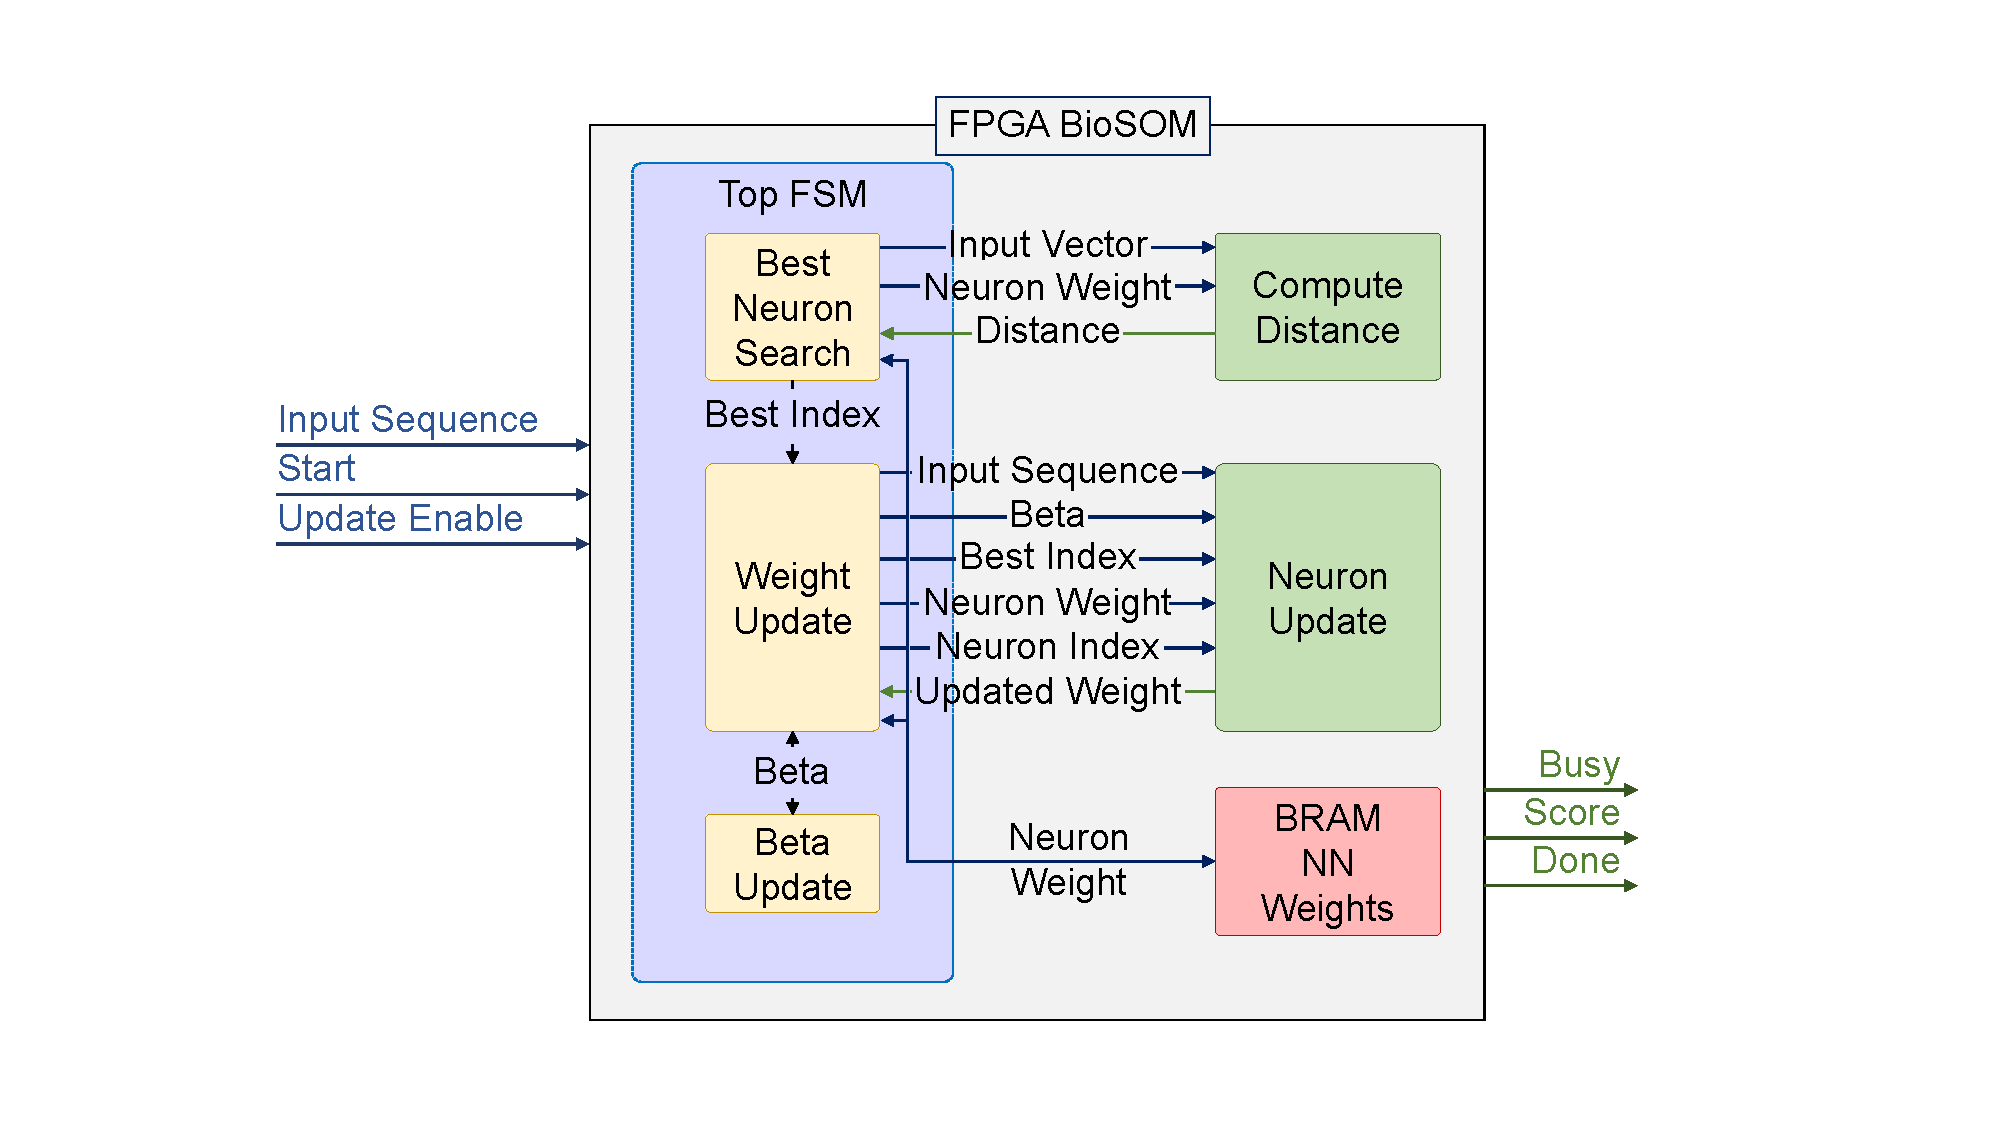
\includegraphics[width=0.49\textwidth]{./somResults/SOMDesignOne_v2}
		\label{fig:algo}}
	\hfil
	\subfloat[]
	{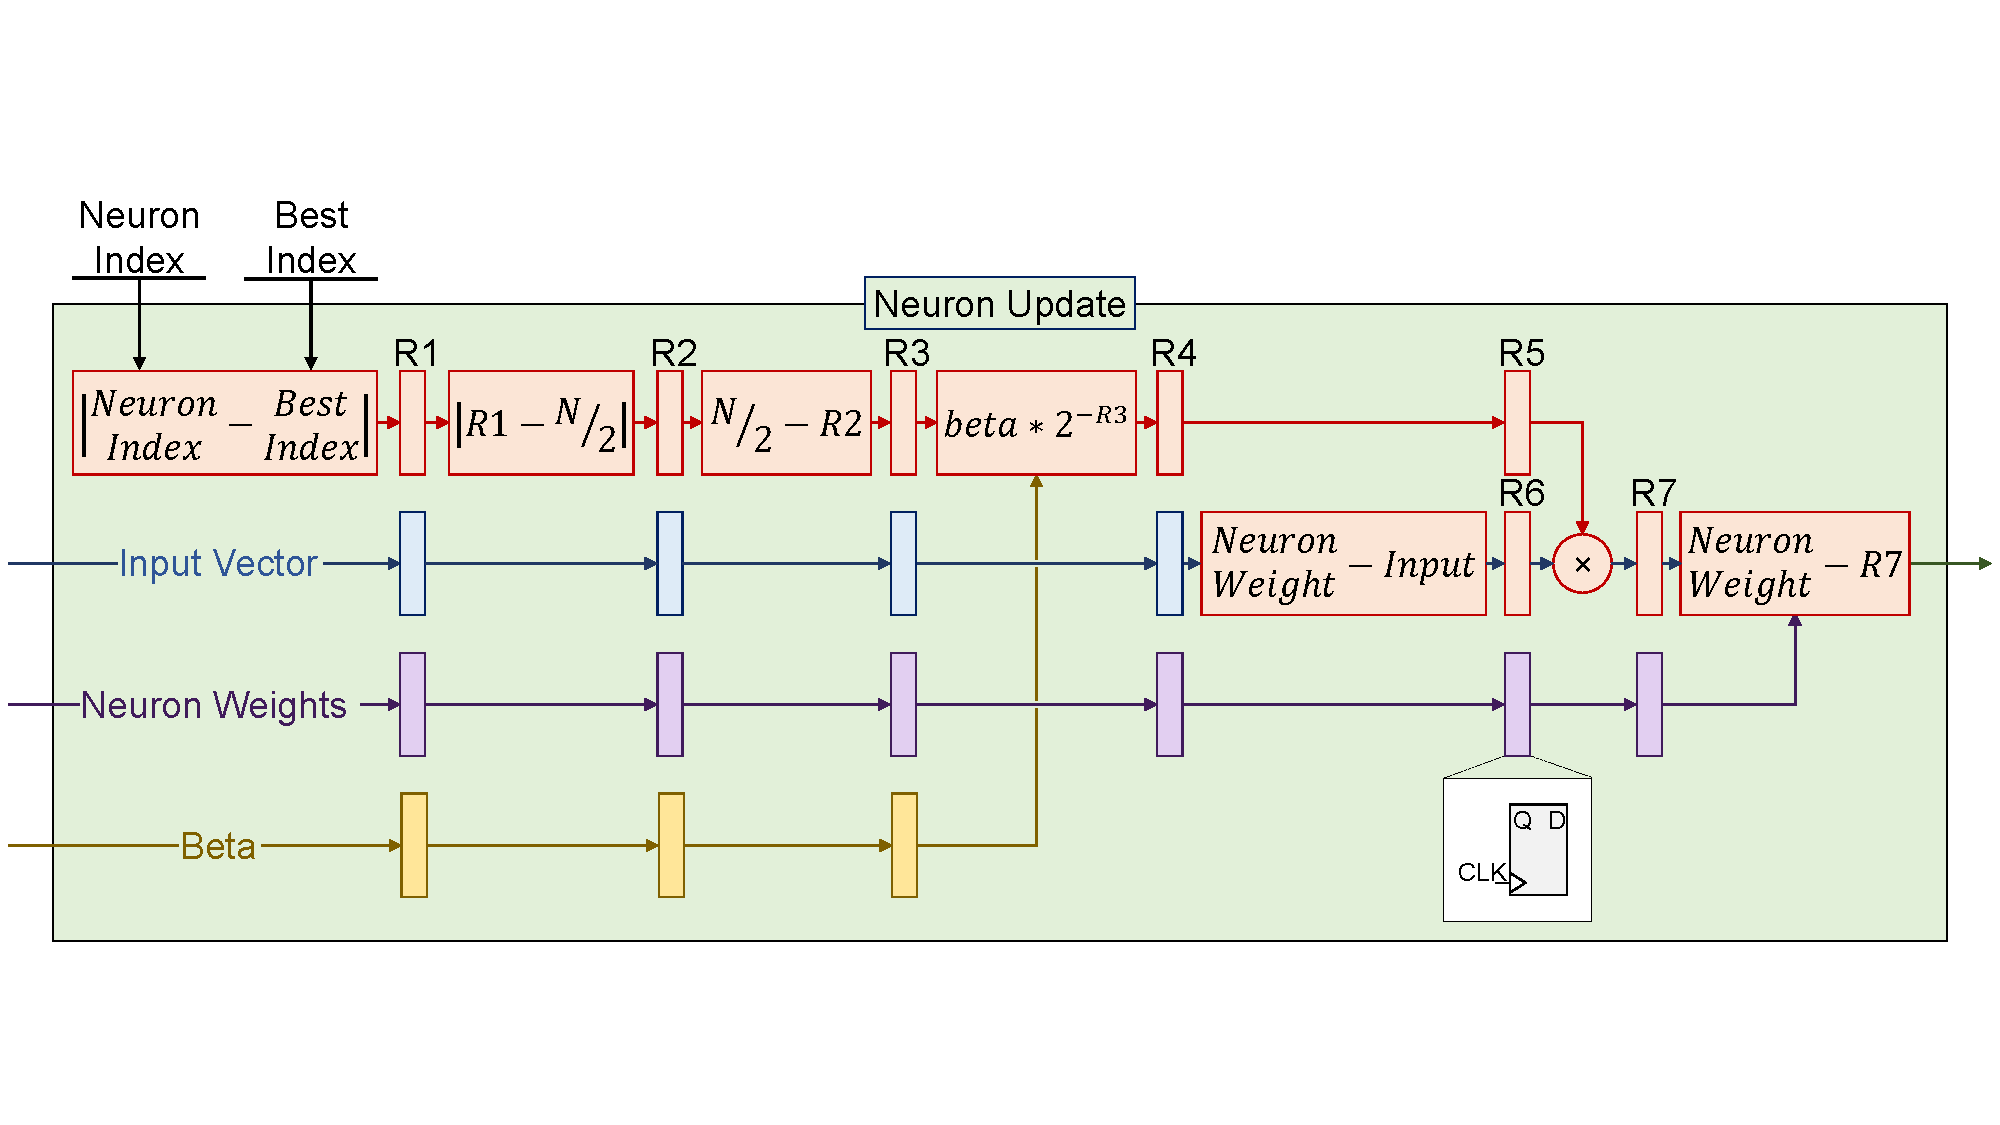
\includegraphics[width=0.49\textwidth]{./somResults/neuronUpdate_v2}
		\label{fig:NeuronUpdate}}
	\caption{(a) Hardware Module for BioSOM. (b) Neuron Update Module.}	\label{fig:SOMFPGAImplementation}
\end{figure}

During the training phase \textit{Neuron Update} component is enabled by setting (\textit{Update Enable=1}). The weights of the Neurons are updated using the distance output of the \textit{Compute Distance} module. The \textit{Neuron Update} component is also pipelined design with II=1. The pipeline stages are shown in Figure \ref{fig:NeuronUpdate}.
\subsection{Results}
The SOM has been implemented with a range of fixed-point formats. With fewer bits, one naturally expects the SOM network to suffer from accuracy degradation. A MATLAB simulation model was created to analyze the accuracy loss when using fixed-point implementation. We trained 10 SOMs with ten different bacteria DNA sequences. Each SOM network has 100 neurons inside, and each neuron has 20 weights. We trained the networks with two independent training processes running in parallel. One is implemented using a double precision floating point, and the other is implemented with fixed-point weights. After training, we used the trained networks to identify the unknown sequence and record their scores.

The FPGA design is implemented with Vivado v.2016.4, used for synthesis and analysis of the HDL Designs. Our design is implemented in VHDL and validated using the Vivado simulator. Experimentation is done for different fixed point representations of weights by modifying parameters in VHDL code. 

The area and power numbers for different weight resolutions are extracted from the reports generated by the Vivado tool post placement and routing with a working frequency of 100 MHz. Table \ref{table:1} compares the resources and area for 8, 12, 16, 24, and 32 bits fixed point formats for a SOM network with 512 neurons. The second part of the table compares the average power in the different fixed point formats for the same SOM.
\begin{table}[!htb]
	\centering
	\caption{Resource Comparison of different fixed point formats}
	\label{table:1}
	\begin{tabular}{ c |c | c| c |c | c } 
		\toprule
		Resource & 8b & 12b & 16b & 24b & 32b \\ 
		\midrule
		LUTs & 1823 & 2611 &3196 & 4375 & 5549 \\
		\hline
		Registers & 3481 & 4679 & 5871 & 8255 & 10639 \\ 
		\hline
		Slice & 854 & 1158 & 1369 &1809 & 2395 \\ 
		\hline
		LUT FF Pairs & 1007 & 1369 & 1750 & 2372 & 3043 \\
		\hline
		B-RAM & 4 & 6 & 8 & 11 & 15 \\
		\hline
		DSP48E1 & 17 & 17 & 17 & 17 & 33 \\
		\hline
		Bonded IOB & 57 & 61 & 65 & 73 & 81 \\
		\midrule
		%    \end{tabular}
	%\end{table}
	
	%\begin{table}[h!]
	%    \centering
	%    \caption{Power Comparison of different fixed-point formats}
	%    \label{table:2}
	%    \begin{tabular}[t]{ c |c | c| c |c | c } 
		\midrule
		Power(W) & 8b & 12b & 16b & 24b & 32b \\ 
		\midrule
		Total Power & 0.295 &0.314 &0.332 &0.356 &0.392 \\
		\hline
		Dynamic &0.052 &0.071 &0.089 &0.113 &0.148 \\ 
		\hline
		Device Static &0.243 &0.243 &0.243 &0.244 &0.244 \\ 
		\bottomrule
	\end{tabular}
\end{table}
\begin{figure}[!htb]
	\centering
    \captionsetup{font=sf}
	\subfloat[]{\includegraphics[width=0.45\textwidth]{./somResults/area}
		\label{fig:area}}
	\hfil
	\subfloat[]{\includegraphics[width=0.45\textwidth]{./somResults/energy}
		\label{fig:energy}}
	\caption{comparison between different fixed-point fromat (a) FPGA LUT utilization (b) energy.}
	\label{fig:metrics}
\end{figure}

The results are summarized in the Figure \ref{fig:area} and \ref{fig:energy}. Both the amount of utilized LUTs and total energy in Joule are presented against the classification error. From the figures, we can easily conclude that we can substantially reduce the resources used and the energy by using a 16-bit fixed-point representation without losing accuracy. We can reduce the resources even further by moving to the 12-bit representation by sacrificing 39\% of the SOM accuracy. 

\section{Conclusion}
With the sudden surge in Neural Network based applications, there is a pressing need to improve the performance and energy efficiency of DNN accelerators for their ubiquitous usage in energy-constrained devices. The performance of DNN accelerators is limited by the memory bandwidth, and off-chip memory accesses dominate the energy consumption. The key to improving the energy efficiency of these NNs is reducing the expensive off-chip memory accesses. Towards this, we proposed approaches to reduce the off-chip memory accesses for DNNs. The proposed approaches improve the data reuse from on-chip memories for CNNs and LSTMs by partitioning the data and scheduling the operations. We have also analyzed the impact of low-bit resolution on the accuracy and energy area performance of NNs. 

\footnotesize
\bibliographystyle{abbrv} %IEEEtran % abbrv
%\vspace{1.5mm}
\bibliography{refs}
%\nocite{*}
%\end{spacing}

\end{document}
